%% LyX 2.2.2 created this file.  For more info, see http://www.lyx.org/.
%% Do not edit unless you really know what you are doing.
%%%%%%%%%%%%%%%%%%%%%%%%%%%%%% User specified LaTeX commands.
%\usepackage{multirow}
%\usepackage{floatrow}

\documentclass[11pt]{article}%
\usepackage[latin9]{inputenc}
\usepackage{amsmath}
\usepackage{amssymb}
\usepackage[authoryear]{natbib}
\usepackage{float}
\usepackage{pdfpages}
\usepackage{graphicx}
\usepackage{amsfonts}
\usepackage{amsthm}
\usepackage{enumerate}
\usepackage{epsfig}
\usepackage{ifthen}
\usepackage{latexsym}
\usepackage{syntonly}
\usepackage{rotating}
\usepackage{lscape}
\usepackage{color}
\usepackage{booktabs}
\usepackage[bottom]{footmisc}
\usepackage{epstopdf}
\usepackage{makeidx}
\usepackage{xr}
% \usepackage{refcheck}%
\setcounter{MaxMatrixCols}{30}
%TCIDATA{OutputFilter=latex2.dll}
%TCIDATA{Version=5.50.0.2960}
%TCIDATA{CSTFile=LaTeX article (bright).cst}
%TCIDATA{LastRevised=Wednesday, August 16, 2023 19:55:35}
%TCIDATA{<META NAME="GraphicsSave" CONTENT="32">}
%TCIDATA{<META NAME="SaveForMode" CONTENT="1">}
%TCIDATA{BibliographyScheme=BibTeX}
%TCIDATA{Language=American English}
%BeginMSIPreambleData
\providecommand{\U}[1]{\protect\rule{.1in}{.1in}}
%EndMSIPreambleData
\textwidth=6.6in
\textheight=8.9in
\headheight=0.0in
\oddsidemargin=0.0in
\headsep=0.0in
\topmargin=0.0in
\newtheorem{theorem}{Theorem}
\newtheorem{corollary}{Corollary}
\newtheorem{case}{Case}
\newtheorem{lemma}{Lemma}
\newtheorem{proposition}{Proposition}
\newtheorem{assumption}{Assumption}
\theoremstyle{definition}
\newtheorem{definition}{Definition}
\newtheorem{example}{Example}
\newtheorem{remark}{Remark}
\def\baselinestretch{1.3}
\newcommand{\abs}[1]{\lvert#1\rvert}
\newcommand{\norm}[1]{\left\lVert#1\right\rVert}
\DeclareMathOperator*{\adjugate}{adj}
\DeclareMathOperator*{\sign}{sgn}
\allowdisplaybreaks
% \externaldocument{Wealth_effect_HARA_Supp_2022}






\begin{document}
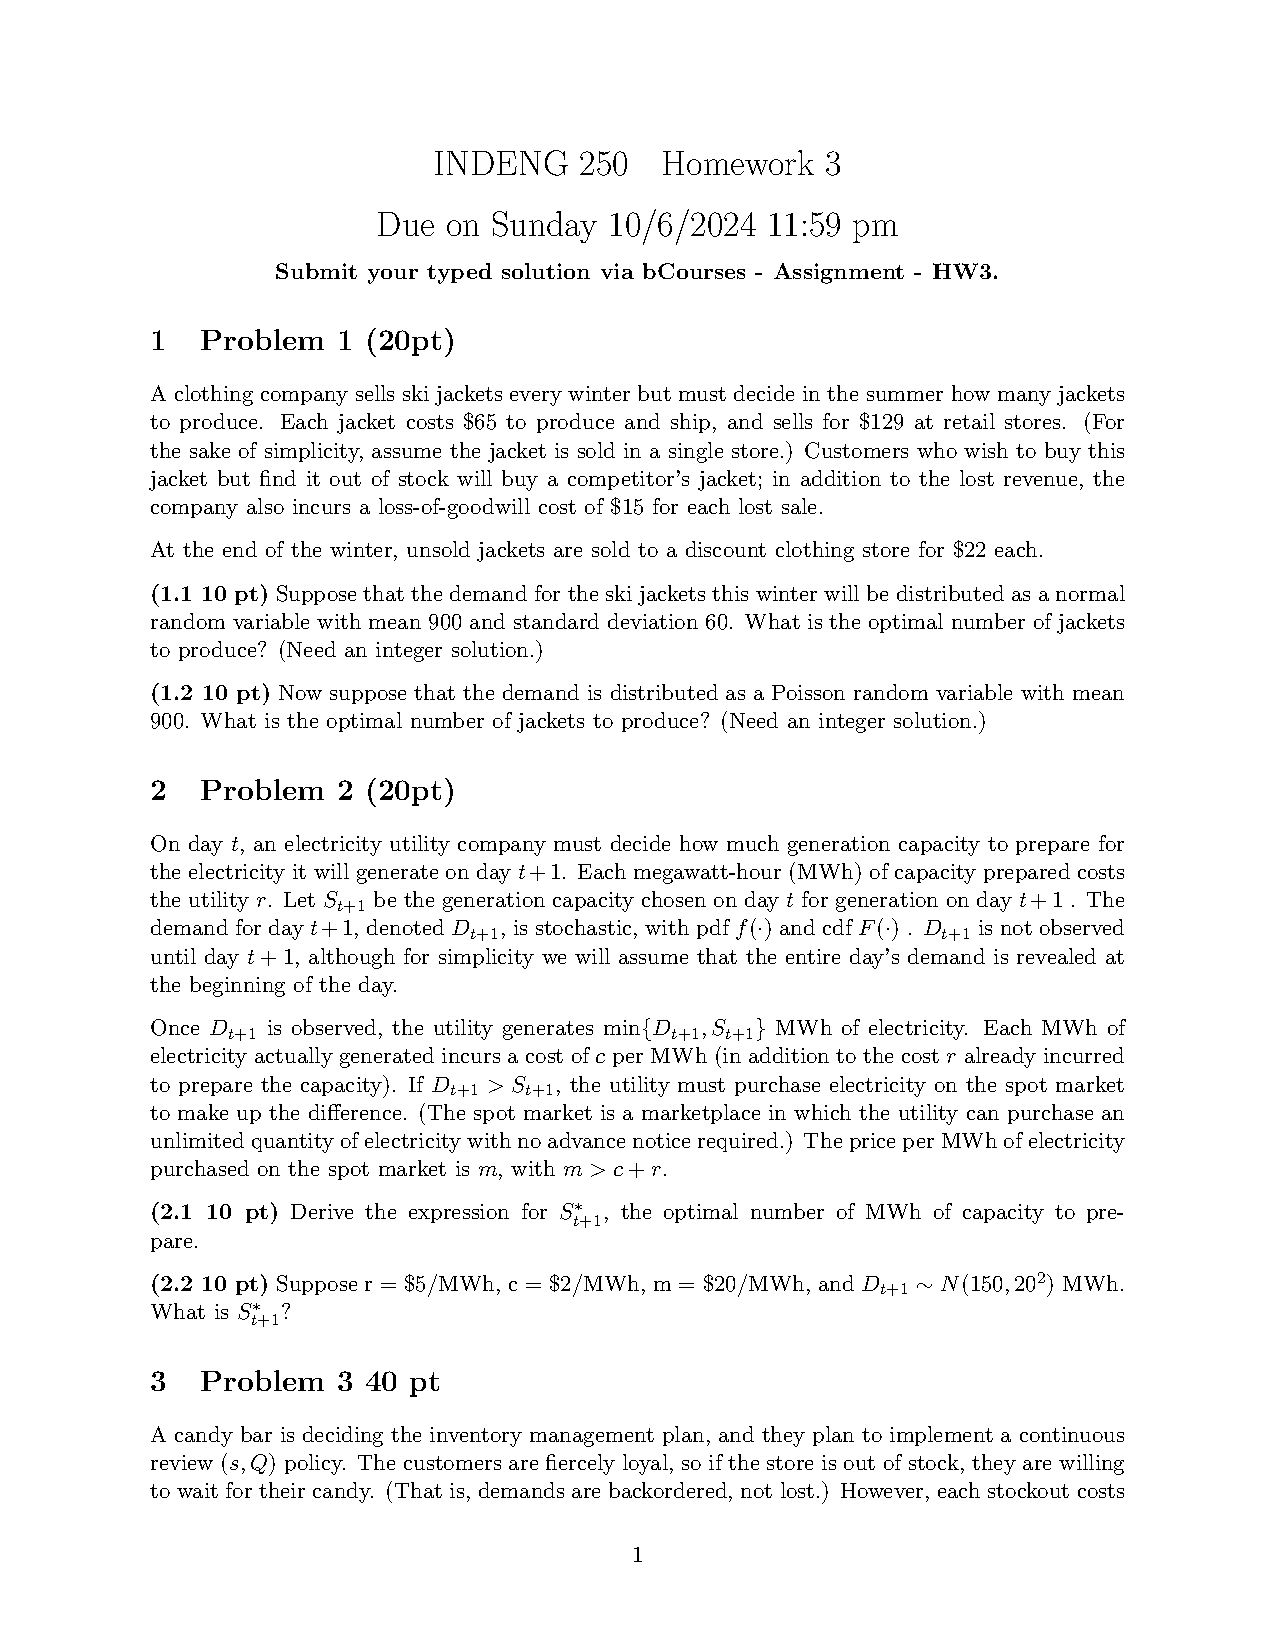
\includepdf[pages={1,2}]{homework3.pdf}
\title{INDENG 250 PS3}
\author{Junyu Guo}
\date{\today }
\maketitle
1. Product cost is 65 and the sell at 129, so the net revenue for each jacket is 64. And if out of stock will lost 15 per jacket from the revenue. And it over the stock then it would cost (65-22)= 43 per jacket.   

1.1 Suppose that the demand for this winter is $Z$, where $Z\sim \mathcal{N}(900,60)$. Now we suppose that we produce $x$ jackets in total. We can categorize the result into the following scenarios. 
\begin{itemize}
    \item $x\geq z$, then the jacket is oversold. The revenue is 
    \begin{equation}
        64 z  -43 (x-z)=107z - 43x.
    \end{equation}
    \item  $x<z$, then the store is out of stock, the revenue is 
    \begin{equation}
        64x - 15(z-x) = 79x - 15z.
    \end{equation}
\end{itemize}
We can represent the result in the form of integrals, suppose the density function of $z$ is $p(z)$.   
\begin{equation}
    f(x) = \int_{-\infty}^x (107z-43x) p(z)dz + \int_{x}^{\infty} (79x-15z)p(z)dz,
\end{equation}
this function is convex with respect to x, therefore we only need to set $\frac{d}{dx}f(x)=0$ and solve the optimal $x^*$. Using the chain rules for derivatives, we can have that 
\begin{equation}
    \frac{d}{dx}f(x)= -43\int_{-\infty}^x p(z)dz + 79\int_{x}^{\infty}p(z)dz =0,
\end{equation}
therefore we can have that 
\begin{equation}
    \operatorname{Pr}(Z\leq x) = \frac{79}{79+43},
\end{equation}
Using the inverse function of normal distribution , we can have that 
\begin{equation}
    x\approx 922.8\approx 923.
\end{equation}
Therefore the production level should be 923.    
1.2 Same as in the first question, we also need to have (where the integrals is only transformed into the summation, so we can obtain the same result).
\begin{equation}
    \operatorname{Pr}(Z\leq x) = \frac{79}{79+43},
\end{equation}
using the distribution probability of the Poisson distribution, we can obtain that 
$x^* = 911 $.        


2. Problem 2      

In the electricity utility example, now we denote the total cost, 
\begin{itemize}
        \item $S_{t+1}\leq D_{t+1}$, then the total cost is 
        \begin{equation}
            C = (c+r) S_{t+1} + m(D_{t+1}-S_{t+1}) 
        \end{equation}
        \item Else, then the total cost should be 
        \begin{equation}
            C = r S_{t+1} + cD_{t+1}.
        \end{equation}
\end{itemize}
Then finally we can write the total cost as , suppose $S_{t+1}=s, $
\begin{equation}
    C(s) = \int_{-\infty}^s (rs+cx )f(x)dx + \int_{s}^{\infty} ((c+r-m)s + mx )f(x)dx.
\end{equation}
To obtain $s^*$, we can set the derivatives of $C(s)$ to be 0 and solve the optimal $s^*$ as 
\begin{equation}
    r \operatorname{Pr}(x\leq s) -(m-c-r)\operatorname{Pr}(x\geq s)=0
\end{equation}
Therefore we can have have 
\begin{equation}
    \operatorname{Pr}(x\leq s)=\frac{m-c-r}{m-c},
\end{equation}
using the definition of accumulated function, we can have 
\begin{equation}
    S_{t+1}^* = F^{-1}(\frac{m-c-r}{m-c}).
    \label{optimal s*}
\end{equation}
2.2 Now we plug the data into (\ref{optimal s*}) and we have that 
$S^*_{t+1} = 161.79$.    

3. Problem 3      
$(s,Q)$ policy   
\begin{itemize}
    \item when to order, when the inventory level falls to $s$
    \item how many items to order: we order a quantity Q
    
\end{itemize}
Fixed cost $K=8$ per order, and purchase $c=0.75$ per unit
The expected cost rate function is 
\begin{equation}
    B(s)\equiv \int_{s}^{\infty} (D_{L}-s)f_{L}(D_{L})dD_{L},
\end{equation}
and the expected backordering cost is 
\begin{equation}
    g(s.Q) = \frac{k\mu}{Q} + h(\frac{Q}{2}+s-\mu L)+\frac{p\mu B(s)}{Q},
\end{equation}
We list the parameters:

\begin{itemize}
    \item $K = 8$
    \item $p=7.5$
    \item $D_{L}\sim \mathcal{N}(108.3,43.3^2)$
    \item $h= 30\%\times 0.75=0.225$
    \item $L = 1/12$
    \item $c = 0.75$
\end{itemize}

    

setting the first derivative to be 0 and we have 
We first compute the EOQ quantity $Q_0 = \sqrt{\frac{2K\mu}{h}}=304$. 
Iteration 1:    
\begin{align}
    s_1 &= F_{L}^{-1}(1-\frac{Q_0h}{p\mu}) = 214.66, \\
    B(s_1) &=  0.099.\\
    Q_1 &= \sqrt{\frac{2\mu[K+pB(s_1)]}{h}} = 318.
\end{align}
Iteration 2:

\begin{align}
    s_2 &= F_{L}^{-1}(1-\frac{Q_1h}{p\mu}) =  213.97, \\
    B(s_2) &= .104\\
    Q_2 &= \sqrt{\frac{2\mu[K+pB(s_2)]}{h}} = 318.51.
\end{align}
Iteration 3:   

\begin{align}
    s_3 &= F_{L}^{-1}(1-\frac{Q_2h}{p\mu}) = 213.93\approx 214  , \\
    B(s_3) &=  .103.\\
    Q_3 &= \sqrt{\frac{2\mu[K+pB(s_3)]}{h}} =  597.67\approx .
\end{align}

Therefore we can obtain that the optimal $s* = 214$ and optimal $Q^* = 598$.    

3.2     Service level = $\operatorname{Pr}(D_{L}\leq s)= 99.2\%$.    

3.3 Now we wish to ensure type-1 service level of 98\%. 
\begin{align*}
    s&= F_{L}^{-1}(1-0.98) = 197.23,\\
    Q &= \sqrt{\frac{2k\mu}{h}}=304. 
\end{align*}

3.4 Now the service level $\beta = 0.98$, 
EOQ quantitiy $Q_0=304$,   $B(s_0)= 0.02\times Q_0= 6.08$ and  $s_0 = 166.88$,    



Iteration 1 : 
\begin{align}
 Q_1 &=\frac{B\left(s_0\right)}{1-F_L\left(s_0\right)}+\sqrt{\frac{2 \mu K}{h}+\left(\frac{B\left(s_0\right)}{1-F_L\left(s_0\right)}\right)^2}=380,\\
 B(s_1) &= 0.02Q_1 =7.6, \\
 S_1 &= 133 .
\end{align}
Iteration 2:
\begin{align}
 Q_2 &=\frac{B\left(s_1\right)}{1-F_L\left(s_1\right)}+\sqrt{\frac{2 \mu K}{h}+\left(\frac{B\left(s_1\right)}{1-F_L\left(s_1\right)}\right)^2}=332,\\
 B(s_1) &= 0.02Q_1=6.64, \\
 S_1 &=136.78 .
\end{align}
Therefore we can have that the optimal $s^* = 37$ and $Q^* = 332$. 

4. In EOQ model, we have the cost function $g(Q)$ as 
\begin{equation}
   g(Q) =  \frac{k\lambda}{Q} + \frac{hQ}{2}, g(Q^{*}) = \sqrt{2K\lambda h }
\end{equation}

suppose the optimal order $\hat{Q} = m Q_B$, then since if we regard the function as a continuouse function it is convex, therefore we only need to make sure that 
\begin{equation}
    f(m )=g(mQ_{B}), f(m)\geq f(m-1) \text{and}
    f(m)\geq f(m+1).
\end{equation}
Using the fact that $f(m)\leq f(m-1)$ and $f(m)\leq f(m+1)$, and we can have that 
\begin{align}
    m(m-1)Q_B^2 \leq (Q^*)^2, m(m+1)Q_B^2 \geq (Q^*)^2,
\end{align}
denote $r = \frac{Q^{*}}{\hat{Q}}$, and we can solve like 
\begin{equation}
    m(m-1)/ m^2\leq  r^2 \leq m(m+1)/m^2,
\end{equation}
taking square root on each term and we can have 
\begin{equation}
    \sqrt{\frac{m-1}{m}}\leq \frac{Q^*}{Q}\leq \sqrt{\frac{m+1}{m}}.
\end{equation}
4.2    

Since we have that for $m\geq 2$, and therefore we have 
\begin{equation}
  \sqrt{  \frac{m}{m+1}}\leq \frac{\hat{Q}}{Q^{*}}\leq\sqrt{ \frac{m}{m-1}},
\end{equation}
and therefore we denote $r = \frac{\hat{Q}}{Q^*}$, and $\sqrt{\frac{2}{3}}\leq r\leq \sqrt{2}$, 
it's easy to observe that 
\begin{equation}
    \frac{g(\hat{Q})}{g(Q^*)} = (r+\frac{1}{r})/2\leq \frac{1}{2}\max\{\frac{3}{\sqrt{2}}, \frac{5}{\sqrt{5}}\}= \frac{3}{\sqrt{2}}/2 =\sqrt{\frac{9}{8}}=1.06, 
\end{equation}
therefore we have solved both 4.2 and 4.3, Q.E.D.
\end{document}